\documentclass{report}

\usepackage{fancyhdr} % Cabeceras de página
\usepackage{lastpage} % Módulo para añadir una referencia a la última página
\usepackage{titling} % No tengo claro para qué es esto
\usepackage[left=3cm,right=2.5cm,top=3cm,bottom=2cm]{geometry} % Márgenes
\usepackage[T1]{fontenc}
\usepackage[utf8x]{inputenc}
\usepackage{xspace}
\usepackage{graphicx}
\usepackage{tikz}
\usepackage{wrapfig}
\usepackage{hyperref}
\usepackage{amssymb}
\usepackage[official]{eurosym}

\hypersetup{
  	hyperindex,
    colorlinks,
    allcolors=blue!60!black
}


\setcounter{secnumdepth}{3}
\renewcommand{\baselinestretch}{1.4}

\title{UAM Software Notification and Damage Management System \\ Project Plan}
\date{\today}
\author{{\Large Triforce} \\ \vspace{5pt} \textit{Iván Márquez Pardo, Víctor de Juan Sanz, Guillermo Julián Moreno}}

\fancyhf{}
\fancypagestyle{plain}{%
	\lhead{\small \itshape Project Plan \, -\, \thedate\, -\, SEPRO}
	\rhead{\vspace{-20pt} 
\includegraphics[width =40 pt]{../Logo.jpg}}
	\cfoot{\thepage\ of \pageref{LastPage}}
	\rfoot{}
}

\begin{document}
\maketitle
\tableofcontents
\newpage
\pagestyle{plain}

\chapter{Requirements and subsystems}
% -*- root: ../ProjectPlan.tex -*-

\newcounter{reqs}[chapter]
\newcommand{\header}[1]{\\ \indent \textbf{#1}\hspace{10pt}}

\newcommand{\reqvertsep}{\vspace{-7pt}}

\newcommand{\reqdesc}{\subparagraph{Description}}
\newcommand{\reqin}{\reqvertsep\subparagraph{Input data}}
\newcommand{\reqout}{\reqvertsep\subparagraph{Output data}}
\newcommand{\reqsteps}{\reqvertsep\subparagraph{Steps}}

\newenvironment{requirement}[1]{
	\stepcounter{reqs}
	\subsection{Requirement \Alph{reqs} - #1}
}{\vspace{20pt}}

\begin{requirement}{Management of priorities categorization}
\reqdesc The system provides a priorities categorization manager which shows the whole list of categories with their assigned priority. 

\reqin Another thing

\reqout Another

\reqsteps The steps go here

\end{requirement}




Before we start defining FML's requirements we need to define two things, the \textbf{roles} inside FML and the \textbf{Operating environment} in which FML will work.


\label{chapRequirements}
\section{Roles}

\paragraph{Reporter role} \label{ReporterRole} This is the role applied to anyone who want to report some fault. It will be taken into account the person's status inside UAM community (student, PhD, teacher, maintenance technician, etc). Every user in FML's system will be able to report faults.

\paragraph{Maintenance Personnel} \label{MaintenancePersonnel}

These are the roles applied to people in charge of maintenance. Inside maintenance personnel we need to distinguish 2 subcategories:

\begin{itemize}
\item Boss: The people in charge of each department.
\item Maintenance technician: The maintenance personnel responsible to fix the faults.
\end{itemize}

As there are 8 departments, there will be 8 categories, listed below:

\begin{itemize}
\item Heating.
\item Plumbing.
\item Air conditioning.
\item Cleaning.
\item Information Technologies.
\item Elevators.
\item Electricity.
\item Trash Collection.
\item Gardeners.
\end{itemize}

Each maintenance person should be tagged in, at least, 1 department. It is also compatible being boss and technician.

\paragraph{Exceptions} The \textbf{cleaning department} only needs a person in charge of the whole department and it is his responsibility to assign faults to their employees and to mark faults as solved.

This department is also special because there is a different department in each faculty, so the must be at least 1 person in charge of each faculty cleaning department. As we mentioned before, maintenance personnel can also report faults.

\paragraph{Administrator Role} Is the person (or group of people) in charge of UAM's maintenance system in general. Every administrator will have permissions to change everything within the application, as they are in charge of everything related with maintenance.

\section{Operating environment}

The main component of Fault Manager Lite is the application, HTML based, that will run in PCs, tablets and smartphones. To improve usability and integration with operating systems, a native application wrapping the HTML interface will be developed so the users won't need to run the browser in order to access the application.

The system will require a backend exposing a RESTful API to which the HTML clients will connect. Separation of concerns is important in order to improve maintainability and ability to respond quickly to user feedback.

The server will require an installation of Python 3, and a working connection to a SQL server. Our application will be independent of the specific implementation of the server (database maintenance will be responsibility of the devops\footnote{I.e., the University's IT team.} team).

Specific implementation details are out of the scope of this proposal, but we will develop the application with scalability in mind: the interface, API and database applications will be independent and loosely coupled in order for the devops team to deploy each one to as many machines as needed. Cloud deployments are an option, but is not required (actually, we recommend using the university datacenter in order to comply with spanish privacy laws).

\section{Requirements}

\subsection{Functional requirements}

\subsubsection{Task Manager subsystem}

\paragraph{Faults definition} Each fault will have 3 possible states: \textit{Pending to assign, assigned, solved}.

If a fault is impossible to be fixed, it will correspond to the administrator to take care personally of it.


\paragraph{Categorizing faults} There should be categories to tag each fault depending on the priority (low, medium or high) and the department who needs to take care of it. The system will assign automatically a priority to each fault, although the administrators will be able to change it at any point in time.

\paragraph{Fault's assignments} FML will assign to maintenance personnel faults to be fixed (depending on the fault's category and maintenance person load of work and capability to solve the fault)

This will be set automatically and the system's administrators will be able to reassign the faults as they pleased.

The person in charge of a department will also be able to reassign faults that have been assigned to his department or to someone inside his department to his employees.

As we mentioned before, the cleaning departments are special, because all cleaning faults in a building will be assign to the person in charge of that building's cleaning.


\paragraph{Task managing} Everyone from the maintenance personnel will have read access to the faults data base through a Graphical User Interface (GUI).

They will just have write access to faults they have been assigned to. \footnote{Write access is needed so the maintenance person change fault's state to \textit{solved} or to \textit{in progress}}

Admin will have write access to all faults in the system, and the person in charge of a department will have write access to all faults assigned to someone inside his department.

\paragraph{When a fault is fixed} The maintenance person assigned (or the manager of that department) will mark as solved the fault. At that time, the reporter will get notify and thanked.


\subsubsection{Report subsystem}

\paragraph{Reporting a fault} Our system will allow:

\begin{itemize}
\item Reporting a fault with the following information: \textit{Location, date, priority\footnote{The actual priority will be set automatically taking into account this priority, the one reported by the user, and other parameters, such as the user's history of reports.}, category, photograph (optional) and description}.

\item See and check reported faults and see its state.

\item Answer questions the maintenance personnel will ask about the reported fault.
\end{itemize}


\paragraph{Duplicated faults} This is a big problem to be solved. What we propose to solve it has 2 aspects.
\begin{itemize}
\item FML will be able to mark as \textit{possible duplicated}, so all possible duplicates will be assign to the same maintenance people, so he can verify if they are duplicated or not.

\item On the other side, to prevent duplicated faults reports, FML will show a message showing possible duplicated faults to the reporter. If the reporter marks the fault he is reporting as duplicated, he will earn some points too and will be added into the list of people to be notified when the task is solved.
\end{itemize}


\subsubsection{Communication subsystem - Notifications and messaging}

\paragraph{Communication} Maintenance person assigned to fix a fault should be able to ask the fault's reporter for more information.

\paragraph{Notifications} All users of the application are able to send an emergency notification which, once revised by the administrator, will appear on the noticeboard of the application of all other users specifying the type of emergency and its location. Among these emergencies, we can find fires or blackouts.

\subsubsection{Users and Profile manager system}

\paragraph{Log in} Everyone must be able to login using UAM credentials. We will use the service provide by UAM to authenticate an user.

If the user is logging in on a smartphone, the system shouldn't ask for the password more than once (except for some specific operations defined in the role-depending requirements, user role category (\ref{Specifics_Secure_Requirements_for_user}))

\paragraph{Updating profile} What if a student become a teacher and then his email needs to be changed? To fix this, every user must be able to update his profile's information.


\subsubsection{Faults History}

\paragraph{Seeing history} As we think transparency is really important, every reporter will be able to see all history of faults. In non-functional requirements we define how this should be done.

\paragraph{Statistics} In the profile page each user should be able to see the faults he has reported and it's state.

Plus, he should be able to see his conversations with maintenance personnel.


\subsection{Non-Functional}

\subsubsection{General Requirements}

This requirements are defined for all roles inside FML (Administrator, maintenance personnel and user)

\paragraph{Profile} Everyone should have a profile with some private information such as name or email.

\paragraph{Lightweight application} FML will be lightweight enough to run in 4 years old Chrome, Firefox, IE's versions.

\paragraph{Read Access to task} Every FML's user will be able to see all reported faults (we think transparency is really important). This will be shown on a map of the UAM. Each fault will appear as an arrow pointing to fault's location and color-tagged depending on its state (solved, pending, assigned).

\subsubsection{Role-depending requirements}

\paragraph{Reporter} FML should provide users the following abilities:
\begin{itemize}
\item The specifics requirements where re-authentication is needed are: \textit{Answering questions asked by maintenance personnel}   \label{Specifics_Secure_Requirements_for_user} and \textit{updating profile information}.
\item The interface to report a fault should be easy enough to let the user report the fault without losing much time.
\item The amount of points earned should be visible inside profiles page. It will be also shown the conversion in ECTS credits so the user knows how much he have earned.

\end{itemize}

\paragraph{Administrator} The administrator should be able to

\begin{itemize}
\item Change the role of a maintenance person.
\item Remove permissions (fault reporting, messaging and/or read access to the fault list) from any user that has misused the application in order to prevent him from misbehaving.
\item Restore permissions (fault reporting, messaging and/or read access to the fault list) to any user that was previously deprived of them.
\item When banning a user, the administrator may choose a period of time: one week, one month, three months, one year, infinite. Once that period has passed, the user will automatically recover his/her permissions.
\end{itemize}

\section{Management of priorities}

\begin{requirement}{Tracking incidence impact}
\reqdesc The system must allow internal users with a maintenance personnel profile to check the impact of the incidences.

\reqin The user logs into the system and selects an incidence.

\reqsteps The system retrieves the incidence from the database, specifically the impact saved.

\reqout The user sees the impact of the incidence.
\end{requirement}


\begin{requirement}{Definition of priority criteria}
\reqdesc The system must allow to specify different criteria to assign automatically a priority to each incidence.

\reqin The user selects parameters of the incidence object and corresponding keywords that will conform the selection criteria, and the desired priority that will be set on match.

\reqsteps The system stores the criteria and applies it automatically on incidence creation in order to establish a priority.

\reqout The system automatically clasifies each incidence based on user-defined criteria: if a certain parameter (e.g., location or description) contains the keywords specificied, the priority will be set to whatever the user specified in the criteria.
\end{requirement}


\begin{requirement}{Management of priorities by personnel in charge}
\reqdesc The personnel in charge of each section must be able to receive reports and manage the incidences based on that information.

\reqin The maintenance personnel sends messages and incidences to the system.

\reqsteps The system saves all the information and shows them to the personnel in charge.

\reqout The personnel in charge of each section sees all related messags and reports.
\end{requirement}


\begin{requirement}{Changes of incidence state}
\reqdesc The personnel in charge of each section must be able to change the state (pending, in process, delayed or resolved) of each incidence.

\reqin The personnel in charge inputs the new state of the incidence.

\reqsteps The system saves the new state.

\reqout The incidence has the new state registered.
\end{requirement}

\begin{requirement}{Changes of incidence category}
\reqdesc The personnel in charge of each section must be able to change the category of each incidence.

\reqin The personnel in charge inputs the new category of the incidence.

\reqsteps The system saves the new category.

\reqout The incidence has the new category registered.
\end{requirement}

\begin{requirement}{Changes of incidence category}
\reqdesc The personnel in charge of each section must be able to change the category of each incidence.

\reqin The personnel in charge inputs the new category of the incidence.

\reqsteps The system saves the new category.

\reqout The incidence has the new category registered.
\end{requirement}


\begin{requirement}{Messaging between users}
\reqdesc The personnel in charge must be able to message the reporter of the incidence.

\reqin The personnel in charge selects the incidence.

\reqsteps The system connects both users.

\reqout Both users can talk between them.
\end{requirement}




\subsection{Management of priorities Categorization}

The system provides a priorities categorization manager which shows the whole list of categories with their assigned priority. 

\begin{requirement}{Filtering list of categories}
\reqdesc The system must allow to search and filter from the category and priority list.

\reqin Value to be searched in the whole list.

\reqout The list filtered by the value given.
\end{requirement}

\begin{requirement}{Add new categories}
\reqdesc  The system must allow to add new categories.
\reqin New category to be created.
\reqout OK or Error message.
\reqsteps Assure the category does not exist previously.
\end{requirement}

\begin{requirement}{Delete categories}
\reqdesc  The system must allow to delete categories.
\reqin Category to be deleted.
\reqout OK or Error message.
\end{requirement}


\begin{requirement}{Modifying stored values}
\reqdesc The system must allow to modify stored values in all attributes
\reqin
\begin{itemize}
\item The attribute to be modified 
\item The new value to be stored.
\end{itemize}

\reqout OK or Error message.
\end{requirement}


\begin{requirement}{List all reports}
\reqdesc The system must allow listing all reported faults.
\reqin Nothing or Category and/or priority to be filtered by.
\reqout List of the reports matching with given values.
\end{requirement}

\begin{requirement}{Consult single report}
\reqdesc The system must allow consulting an single report's aspects.
\reqin Selection of a report.
\reqout The information stored of the selected report.
\end{requirement}

\begin{requirement}{Modify single report's priority}
\reqdesc The system must allow modifying the priority given to a single report.
\reqin \begin{itemize}
\item The report to be updated.
\item The new priority to be stored.
\end{itemize}
\reqout OK or Error message.

\end{requirement}





% -*- root: ../ProjectPlan.tex -*-
\section{Project Definition}

FML is based on the jolly cooperation between the users of the facilities of the UAM campus and the maintenance staff in charge of them.

As the users will be the ones that will detect the sooner faults on the facilities the campus offers them, they are also the most suitable to report the problems they are having, in order to getting them fixed as soon as possible. With the FML web application, it will only take less than a minute to fill the form and send it to the maintenance staff.

Using the reports of faults detected in the campus, the maintenance personnel will stop losing its precious time revising the installations looking for faults and will be able to focus on the repairs. Apart from this benefit, the maintenance staff will also have a better way to coordinate efforts, as the FML will provide an automatic assignment system to assign repairs to each of the members avoiding overloading any of them and taking into account their distance to the problem, saving time on displacements.

In summary, the users will be able to easily report faults on facilities they are using in order to have them fixed in the less time possible, while the maintenance personnel will multiply its current performance as the majority of their resources will stop being wasted on revisions, but on repairs. 

\section{Breakdown in Subsystems}

\begin{figure}[hbtp]
\centering
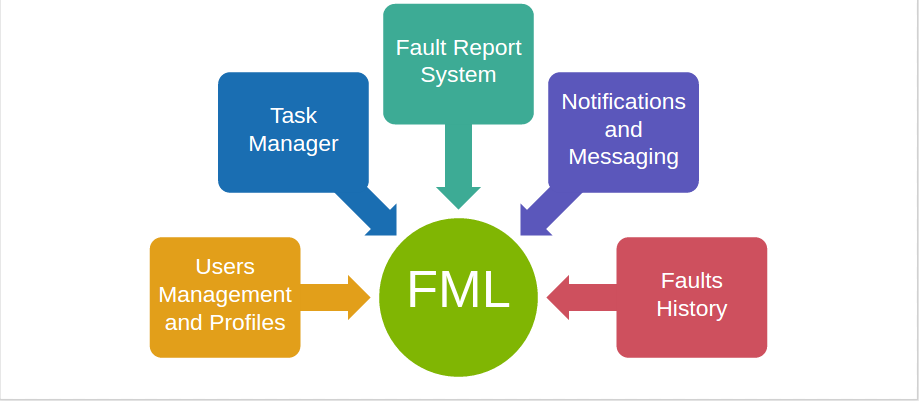
\includegraphics[scale=0.5]{img/subsystems.png}
\caption{Schematic for the subsystems of the project.}
\label{figSubsystems}
\end{figure}

In order to achieve the goals described in chapter \ref{chapIntroduction}, the Fault Manager Lite application is divided into five subsystems: \emph{Task Management}, \emph{Report System}, \emph{Notification and Messaging System}, \emph{User Management} and \emph{Faults History and Statistics}, as seen in figure \ref{figSubsystems}.

A brief description of the functionalities of each mentioned subsystem can be found in the next sections of the document.

\subsection{Task Management}
\label{subsection Task Management}

This subsystem is in charge of the management of repair tasks, which are automatically generated whenever the system receives a new fault report.

Users will use the report system of the application (see \ref{subsection Report System}) to send report faults. These faults will be analyzed by this subsystem and automatically classified depending on their department and priority. Then, their corresponding repair task will be generated based on the form filled by the user and assigned to the closest technician depending on the location of the fault.

Managers will be able to change manually the priority and the person in charge of repairing that fault, which are automatically assigned by the subsystem. The category of the fault can also be modified in case it is not correct; in that case, the fault will then be sent to the manager of the new department. Cleaning department will be treated differently as there is a manager for each building of the UAM campus, so cleaning tasks will be assigned to those managers taking into account this characteristic.

Technicians who have been assigned a repair task will be notified (see \ref{subsection Notification and Messaging System}) and be able to consult the information related to that task. This task information includes: ID of the reporter, location of the fault, timestamp of the report, brief description (subject), detailed description, category, status, priority and occasionally a photography (if any was given by the reporter).

The status of a fault can be: \emph{Pending} (just received by the system, before having been automatically assigned by the system or manually assigned by a manager), \emph{Assigned} (already assigned to a technician, who is or will be eventually solving it) or \emph{Solved} (the task has been successfully completed as the fault has been repaired). Technicians will be able to change the current status of a task assigned to them in order to give managers real-time information about the status of faults' troubleshooting.

Managers will also be able to consult real-time information about repair tasks assigned to members of their departments and make reassignments of tasks in case, for example, of overloading a certain technician or in order to accelerate an specific repair.

\subsection{Report System}
\label{subsection Report System}

This subsystem is in charge of the fault report system, which is the main and most important activity of the whole software system.

Whenever users and/or technicians encounter a fault on the facilities of the campus, they will be able to fill a form in order to report that fault and accelerate its troubleshooting. This fault will then be sent to the FML server, which will assign its repair task to the corresponding technician (see \ref{subsection Task Management}).

The mandatory fields of the form include: a brief description of the problem (subject), a more detailed description (1000 characters maximum length), category (department of the maintenance service) and location (which can be automatically set using GPS technology or manually set by the user in case the GPS function doesn't work properly). The ID of the reporter and the timestamp of the report will be automatically added before sending it.

As an optional field, users can add a photography to their report in case they want to be more specific. The photo will be taken on the fly or added from the user's gallery.

After sending a fault report, the reporter will be able to consult the real-time status of its repair task by selecting that task from his/her fault history (see \ref{subsection Fault History and Statistics}). Reporting a fault enables the opening of a chat conversation with the technician assigned to the repair (see \ref{subsection Notification and Messaging System}).

The report system is also in charge of analyzing newly received fault reports and determine if they can be duplicates of existing reports, by comparing their characteristics: location, similar timestamps and same keywords in the descriptions. Potential duplicates will be sent to the manager, who will decide if they really are the same issue or not.

\subsection{Notification and Messaging System}
\label{subsection Notification and Messaging System}
This subsystem is the one in charge of sending and receiving notifications and messages from the application.

There will exist general and emergency notifications (such as special events in the campus and a fire or blackout in a building, respectively). This notifications will only be sent by managers and all the users will receive that alerts.

Technicians will receive a notification informing them of their assignment of a new task. They will also be able to establish a communication channel (private chat) with the reporter of a fault, in order to ask for more information about that fault. Users will not be able to open this communication channel with the technician in charge of their reported fault, while managers will be able to open a private chat with any member of their departments for a better management and organization of them.

When a fault is repaired and the technician changes its status to solved (see \ref{subsection Task Management}), its reporter will receive a notification about the finish of the repair.

Users and technicians will be able to delete messages or notifications they have received.

\subsection{User Management}
\label{subsection User Management}

This subsystem is in charge of several issues related to the application users, including login, user profile and user's fault history.

In this section, the term `user' will make reference to every member of the UAM that uses the FML application as a reporter or as a member of the maintenance service.

When entering the application, users must introduce their credentials for accessing the UAM's web services. Those credentials will be sent to the UAM members server, which will inform the FML server about the correctness (or not) of them. Login credentials will only be needed once (the first time you access to the application).

Every user will have a profile, including some (optionally filled) information about them. From this profile, every user will have access to their fault report history; every report can be selected in order to see its current status (see \ref{subsection Fault History and Statistics}).

In case of students, this profile will also show them information about their current progress in the achievement of optional credits as a reward for their report history.

This system is also in charge of filtering and/or searching for users in the database. This ability to look for users in the database is only accessible to managers.

\subsection{Fault History and Statistics}
\label{subsection Fault History and Statistics}

This subsystem is in charge of several activities related to fault reports, including their search and the generation of statistics related to them.

When a fault is reported (see \ref{subsection Report System}), that report is saved in the database and its entry can be eventually change. For example, its status will be eventually changed when it gets repaired by a technician, it can be assigned to another technician or its priority can be modified by a manager (see \ref{subsection Task Management}).

Managers will be able to consult the fault database to look for all its entries or apply some filters to look for specific faults. Among the filters that can be applied in the search, there are: category/department, date range, reporter, technician or keyword in the description.

User profiles will make accessible information about fault reports related to those users: reporters will see the faults they have reported and their real-time status, while technicians will see the faults they have repaired or have been assigned to do so. Managers will have all this information available by applying the corresponding filter.

Managers will also be able to generate statistics based on the fault history contained in the database. This statistics can be general, related to their departments or related to a member of their technical staff. The generated statistics can be used to analyze the troubleshooting efficiency of the maintenance service or detect problematic areas.

Users will be able to see a simplified map of the campus with colored signs on it. Each dot represents a reported fault and the color will follow a color code, making its status easily distinguishable depending on it: Pending to assign (red), Assigned (yellow) and Solved (Solved). Only the last 30 reports will be shown in this map at the same time to ensure their visibility.



\chapter{System size estimation}
% -*- root: ../ProjectPlan.tex -*-
Estimations of time and complexity of the system are basic in order to make a project plan adjusted to the real development time. On the contrary, we won't have any basis to aproximate that time, depending just on a correct planification guided by previous experiences.

With this aim, the size of the Fault Manager Lite project has been estimated using the Function Points estimation technique. Moreover, we have also estimated the Report System (subsystem of FML) with the COCOMO II tool.

\section{Estimation using function points}
\subsection{Unadjusted Function Points}
After the evaluation of the requirements of the proposed system using the Function Points analysis, we have obtained the data of its estimated complexity. We attach tables with the size of the different subsystems in which the application is divided into, with their corresponding estimations in terms of Function Points. For a more detailed analysis of each of the exposed requirements, see \ref{chapFunctionPoints}.


\subsubsection{Task Management Subsystem}
Table \ref{tbl_TMS_UFP} shows the summary of the unadjusted Function Points calculated for the Task Management Subsystem.
\begin{table}[hbtp]
\centering

\begin{tabular}{|l|c|c|c|c|c|c|c|}
\cline{2-7}
\multicolumn{1}{c}{} & \multicolumn{6}{|c|}{\textsc{Complexity}} & \multicolumn{1}{c}{}  \\ \cline{2-8}
\multicolumn{1}{c|}{} & \textbf{Low} & \textbf{Medium} & \textbf{High} & \textbf{Low} & \textbf{Medium} & \textbf{High} & \multirow{2}{*}{\textit{Unadjusted FP}} \\ \cline{1-7}
\textbf{Data fns.} & \multicolumn{3}{|c|}{\textit{Frequency}} &  \multicolumn{3}{|c|}{\textit{Weight}} & \\ \hline
ILF 	& 11 & 0 & 0 & 7 & 10 & 15 & 77 	\\ \hline
EIF 	& 0 & 0 & 0 & 5 & 7 & 10 & 0		\\ \hline
\textbf{Transactional fns.} & \multicolumn{7}{|c|}{} \\ \hline
EI 		& 0 & 0 & 0 & 3 & 4 & 6 & 0 		\\ \hline
EO 		& 0 & 0 & 0 & 4 & 5 & 7 & 0		\\ \hline
EQ		& 3 & 0 & 0 & 3 & 4 & 6 & 9		\\ \hline
\multicolumn{6}{c|}{} & \textbf{Total} & 86.0 \\ \cline{7-8}
\end{tabular}

\caption{Overview of the calculation of the Unadjusted Function Points for the Task Management Subsystem.}
\label{tbl_TMS_UFP}
\end{table}

\subsubsection{Report System Subsystem}
Table \ref{tbl_RSS_UFP} shows the summary of the unadjusted Function Points calculated for the Report System Subsystem.
\begin{table}[hbtp]
\centering

\begin{tabular}{|l|c|c|c|c|c|c|c|}
\cline{2-7}
\multicolumn{1}{c}{} & \multicolumn{6}{|c|}{\textsc{Complexity}} & \multicolumn{1}{c}{}  \\ \cline{2-8}
\multicolumn{1}{c|}{} & \textbf{Low} & \textbf{Medium} & \textbf{High} & \textbf{Low} & \textbf{Medium} & \textbf{High} & \multirow{2}{*}{\textit{Unadjusted FP}} \\ \cline{1-7}
\textbf{Data fns.} & \multicolumn{3}{|c|}{\textit{Frequency}} &  \multicolumn{3}{|c|}{\textit{Weight}} & \\ \hline
ILF 	& 1 & 0 & 0 & 7 & 10 & 15 & 7 	\\ \hline
EIF 	& 0 & 0 & 0 & 5 & 7 & 10 & 0		\\ \hline
\textbf{Transactional fns.} & \multicolumn{7}{|c|}{} \\ \hline
EI 		& 2 & 0 & 0 & 3 & 4 & 6 & 6		\\ \hline
EO 		& 0 & 0 & 0 & 4 & 5 & 7 & 0		\\ \hline
EQ		& 0 & 0 & 0 & 3 & 4 & 6 & 0		\\ \hline
\multicolumn{6}{c|}{} & \textbf{Total} & 13.0 \\ \cline{7-8}
\end{tabular}

\caption{Overview of the calculation of the Unadjusted Function Points for the Report System Subsystem.}
\label{tbl_RSS_UFP}
\end{table}

\subsubsection{Notification and Messaging System Subsystem}
Table \ref{tbl_NMSS_UFP} shows the summary of the unadjusted Function Points calculated for the Notification and Messaging System Subsystem.
\begin{table}[hbtp]
\centering

\begin{tabular}{|l|c|c|c|c|c|c|c|}
\cline{2-7}
\multicolumn{1}{c}{} & \multicolumn{6}{|c|}{\textsc{Complexity}} & \multicolumn{1}{c}{}  \\ \cline{2-8}
\multicolumn{1}{c|}{} & \textbf{Low} & \textbf{Medium} & \textbf{High} & \textbf{Low} & \textbf{Medium} & \textbf{High} & \multirow{2}{*}{\textit{Unadjusted FP}} \\ \cline{1-7}
\textbf{Data fns.} & \multicolumn{3}{|c|}{\textit{Frequency}} &  \multicolumn{3}{|c|}{\textit{Weight}} & \\ \hline
ILF 	& 1 & 0 & 0 & 7 & 10 & 15 & 7 	\\ \hline
EIF 	& 0 & 0 & 0 & 5 & 7 & 10 & 0		\\ \hline
\textbf{Transactional fns.} & \multicolumn{7}{|c|}{} \\ \hline
EI 		& 0 & 0 & 0 & 3 & 4 & 6 & 0 		\\ \hline
EO 		& 0 & 0 & 0 & 4 & 5 & 7 & 0		\\ \hline
EQ		& 3 & 0 & 0 & 3 & 4 & 6 & 9		\\ \hline
\multicolumn{6}{c|}{} & \textbf{Total} & 16.0 \\ \cline{7-8}
\end{tabular}

\caption{Overview of the calculation of the Unadjusted Function Points for the Notification and Messaging System Subsystem.}
\label{tbl_NMSS_UFP}
\end{table}

\subsubsection{User Management Subsystem}
Table \ref{tbl_UMS_UFP} shows the summary of the unadjusted Function Points calculated for the User Management Subsystem.
\begin{table}[hbtp]
\centering

\begin{tabular}{|l|c|c|c|c|c|c|c|}
\cline{2-7}
\multicolumn{1}{c}{} & \multicolumn{6}{|c|}{\textsc{Complexity}} & \multicolumn{1}{c}{}  \\ \cline{2-8}
\multicolumn{1}{c|}{} & \textbf{Low} & \textbf{Medium} & \textbf{High} & \textbf{Low} & \textbf{Medium} & \textbf{High} & \multirow{2}{*}{\textit{Unadjusted FP}} \\ \cline{1-7}
\textbf{Data fns.} & \multicolumn{3}{|c|}{\textit{Frequency}} &  \multicolumn{3}{|c|}{\textit{Weight}} & \\ \hline
ILF 	& 2 & 0 & 0 & 7 & 10 & 15 & 14 	\\ \hline
EIF 	& 1 & 0 & 0 & 5 & 7 & 10 & 5		\\ \hline
\textbf{Transactional fns.} & \multicolumn{7}{|c|}{} \\ \hline
EI 		& 0 & 0 & 0 & 3 & 4 & 6 & 0 		\\ \hline
EO 		& 0 & 0 & 0 & 4 & 5 & 7 & 0		\\ \hline
EQ		& 3 & 0 & 0 & 3 & 4 & 6 & 9		\\ \hline
\multicolumn{6}{c|}{} & \textbf{Total} & 28.0 \\ \cline{7-8}
\end{tabular}

\caption{Overview of the calculation of the Unadjusted Function Points for the User Management Subsystem.}
\label{tbl_UMS_UFP}
\end{table}

\subsubsection{Faults History and Statistics Subsystem}
Table \ref{tbl_FHSS_UFP} shows the summary of the unadjusted Function Points calculated for the Faults History and Statistics Subsystem.
\begin{table}[hbtp]
\centering

\begin{tabular}{|l|c|c|c|c|c|c|c|}
\cline{2-7}
\multicolumn{1}{c}{} & \multicolumn{6}{|c|}{\textsc{Complexity}} & \multicolumn{1}{c}{}  \\ \cline{2-8}
\multicolumn{1}{c|}{} & \textbf{Low} & \textbf{Medium} & \textbf{High} & \textbf{Low} & \textbf{Medium} & \textbf{High} & \multirow{2}{*}{\textit{Unadjusted FP}} \\ \cline{1-7}
\textbf{Data fns.} & \multicolumn{3}{|c|}{\textit{Frequency}} &  \multicolumn{3}{|c|}{\textit{Weight}} & \\ \hline
ILF 	& 0 & 0 & 0 & 7 & 10 & 15 & 0 	\\ \hline
EIF 	& 0 & 0 & 0 & 5 & 7 & 10 & 0		\\ \hline
\textbf{Transactional fns.} & \multicolumn{7}{|c|}{} \\ \hline
EI 		& 0 & 0 & 0 & 3 & 4 & 6 & 0 		\\ \hline
EO 		& 0 & 3 & 0 & 4 & 5 & 7 & 15		\\ \hline
EQ		& 6 & 0 & 0 & 3 & 4 & 6 & 18		\\ \hline
\multicolumn{6}{c|}{} & \textbf{Total} & 33.0 \\ \cline{7-8}
\end{tabular}

\caption{Overview of the calculation of the Unadjusted Function Points for the Faults History and Statistics Subsystem.}
\label{tbl_FHSS_UFP}
\end{table}

\subsubsection{Global Estimation}
Table \ref{tbl_GLOBAL_UFP} shows the summary of the unadjusted Function Points of the whole system, given by the sum of the unadjusted FP of each subsystem.
\begin{table}[hbtp]
\centering

\begin{tabular}{|l|c|c|c|c|c|c|c|}
\cline{2-7}
\multicolumn{1}{c}{} & \multicolumn{6}{|c|}{\textsc{Complexity}} & \multicolumn{1}{c}{}  \\ \cline{2-8}
\multicolumn{1}{c|}{} & \textbf{Low} & \textbf{Medium} & \textbf{High} & \textbf{Low} & \textbf{Medium} & \textbf{High} & \multirow{2}{*}{\textit{Unadjusted FP}} \\ \cline{1-7}
\textbf{Data fns.} & \multicolumn{3}{|c|}{\textit{Frequency}} &  \multicolumn{3}{|c|}{\textit{Weight}} & \\ \hline
ILF 	& 15 & 1 & 0 & 7 & 10 & 15 & 115 	\\ \hline
EIF 	& 1  & 0 & 0 & 5 & 7 & 10 & 5		\\ \hline
\textbf{Transactional fns.} & \multicolumn{7}{|c|}{} \\ \hline
EI 		& 2  & 0 & 0 & 3 & 4 & 6 & 6 		\\ \hline
EO 		& 0  & 3 & 0 & 4 & 5 & 7 & 15		\\ \hline
EQ		& 15 & 0 & 0 & 3 & 4 & 6 & 45		\\ \hline
\multicolumn{6}{c|}{} & \textbf{Total} & 186.0 \\ \cline{7-8}
\end{tabular}

\caption{Overview of the calculation of the Unadjusted Function Points for the whole system.}
\label{tbl_GLOBAL_UFP}
\end{table}

\emph{The number of Unadjusted Function Points of the system is 186.}


\subsection{Adjusting Factor}
Once the unadjusted Function Points of the project have been calculated, these must be ponderated depending of the technical characteristics of the system. To do this, we have evaluated the 14 adjusting characterístics involved in the Function Points method in order to extract the Adjusting Factor for this system.

Table \ref{tbl_ADJ_FACTOR} shows the summary of the values assigned to the general characteristics of the system.

\begin{table}[hbtp]
\centering

\begin{tabular}{l|c}
\textbf{Complexity Factors} & \textbf{Value} \\ \hline
Data communication & 4 \\
Distributed functions & 3 \\
Performance & 1 \\
Strongly used configurations & 2 \\
Transactions frequency & 4 \\
Online data input & 4 \\
Design for the efficiency of the final user & 3 \\
Online update & 3 \\
Complex processes & 3 \\
Other systems utilization & 3 \\
Installation ease & 5 \\
Operation ease & 2 \\
Multiple sites instalation & 3 \\
Change ease & 5 \\ \hline
\textit{TOTAL DEGREE OF INFLUENCE (TDI)} & \textit{45.0}
\end{tabular}
\caption{Complexity Factor values.}
\label{tbl_ADJ_FACTOR}
\end{table}

Therefore, the TDI is 45.0. The Adjusting Factor (AF) is calculated applying the corresponding formula:
\emph{AF = (TDI x 0.01) + 0.65 = 1.10}

\emph{The Adjusting Factor of the system is 1.10.}

\subsection{Adjusted Function Points}
Once we have obtained the Unadjusted Function Points, UFP, and the Adjusting Factor, AF, we have that the Adjusted Function Points, AFP, are:
\emph{AFP = UFP x AF}

This way, we have that the AFP of each subsystem, as well as the total AFP for the project are the ones exposed in Table \ref{tbl_GLOBAL_AFP}.

\begin{table}[hbtp]
\centering

\begin{tabular}{l|c|c}
\textbf{Subsystem} & \textbf{UFP} & \textbf{AFP} \\ \hline
Task Management	& 93.0 & 102.3 \\
Report System & 13.0 & 14.3 \\
Notification and Messaging System & 16.0 & 17.6 \\
User Management & 28.0 & 30.8 \\
Faults History and Statistics & 33.0 & 36.3 \\ \hline
\textit{Total} & \textit{183.0} & \textit{201.3}
\end{tabular}
\caption{Adjusted Function Points organized by subsystems.}
\label{tbl_GLOBAL_AFP}
\end{table}


\subsection{Time Estimation}

Taking into account all the elements shown in the tables of the previous section and that every Adjusted Function Point implies an estimated effort of \textbf{1.615 person-day}, then we can estimate the time needed to develop every subsystem, and therefore, the whole system itself.

The next tables show a summary for every subsystem estimated time:

\begin{table}[hbtp]
\centering
\begin{tabular}{l|c}
\textbf{Summary} & \textbf{Value} \\ \hline
Raw function points (FP) & 93 \\
Complexity factor (CF) & 45 \\
Adjustment factor & 1.10 \\
Adjusted function points & 102.3 \\
Person/day per function points & 1.466 \\ \hline
\textit{Estimated person-days} & \textit{149.972}
\end{tabular}

\caption{Estimated size (person-day) for the Task Management subsystem.}
\end{table}

\begin{table}[hbtp]
\centering
\begin{tabular}{l|c}
\textbf{Summary} & \textbf{Value} \\ \hline
Raw function points (FP) & 13 \\
Complexity factor (CF) & 45 \\
Adjustment factor & 1.10 \\
Adjusted function points & 14.3 \\
Person/day per function points & 1.615 \\ \hline
\textit{Estimated person-days} & \textit{23.0945}
\end{tabular}

\caption{Estimated size (person-day) for the Report System subsystem.}
\end{table}

\begin{table}[hbtp]
\centering
\begin{tabular}{l|c}
\textbf{Summary} & \textbf{Value} \\ \hline
Raw function points (FP) & 16 \\
Complexity factor (CF) & 45 \\
Adjustment factor & 1.10 \\
Adjusted function points & 17.6 \\
Person/day per function points & 1.466 \\ \hline
\textit{Estimated person-days} & \textit{25.80}
\end{tabular}

\caption{Estimated size (person-day) for the Notification Messaging subsystem.}
\end{table}

\begin{table}[hbtp]
\centering
\begin{tabular}{l|c}
\textbf{Summary} & \textbf{Value} \\ \hline
Raw function points (FP) & 28 \\
Complexity factor (CF) & 45 \\
Adjustment factor & 1.10 \\
Adjusted function points & 30.8 \\
Person/day per function points & 1.615 \\ \hline
\textit{Estimated person-days} & \textit{49.742}
\end{tabular}

\caption{Estimated size (person-day) for the User Management subsystem.}
\end{table}

\begin{table}[hbtp]
\centering
\begin{tabular}{l|c}
\textbf{Summary} & \textbf{Value} \\ \hline
Raw function points (FP) & 33 \\
Complexity factor (CF) & 45 \\
Adjustment factor & 1.10 \\
Adjusted function points & 36.3 \\
Person/day per function points & 1.466 \\ \hline
\textit{Estimated person-days} & \textit{53.2158}
\end{tabular}

\caption{Estimated size (person-day) for the Fault History and Statistics subsystem.}
\end{table}

\begin{table}[hbtp]
\centering
\begin{tabular}{l|c}
\textbf{Summary} & \textbf{Value} \\ \hline
Raw function points (FP) & 183 \\
Complexity factor (CF) & 45 \\
Adjustment factor & 1.10 \\
Adjusted function points & 201.3 \\
Person/day per function points & 1.466 \\ \hline
\textit{Estimated person-days} & \textit{295.1058}
\end{tabular}

\caption{Estimated size (person-day) for the whole FML system.}
\label{tbl_FPEstimation}
\end{table}

Tables \ref{tbl_GLOBAL_UFP} and \ref{tbl_FPEstimation} detail the estimation of the project size and time required for its completion based on the method of function points.

Based on these calculations, the project would consist of approximately 207 adjusted function points. That would translate to 330.429 person-days of development time.

\subsection{Estimation using CoCoMo II method}

I don't know how to use Cocomo to estimate size.



\chapter{Project plan}
% -*- root: ../ProjectPlan.tex -*-

\section{Gantt diagram}

\section{Resources and activities assignment}

\section{Estimation of development costs}

\begin{table}[hbtp]
\centering
\begin{tabular}{l|ccccc|c}
\multirow{2}{*}{\textbf{Phase}} & \textbf{Effort} & \textbf{Labour} & \textbf{Running} & \textbf{Fixed} & \textbf{Total} & \textbf{Duration} \\
& \textit{Person-months} & \textit{K\$} & \textit{K\$ / month} & \textit{K\$} & \textit{K\$} & \textit{Months} \\
\textsc{Requirements} & 0.1 & 0.8 & 1.05 & 0 & 1.535 & 0.7 \\
\textsc{Product design} & 0.3 & 1.5 & 1.05 & 0 & 2.55 & 1 \\
\textsc{Detailed design} & 0.4 & 2.3 & 1.05 & 0 & 3.35 & 1 \\
\textsc{Code \& Unit tests} & 0.5 & 2.8 & 1.05 & 8.25 & 12.415 & 1.3 \\
\textsc{Integration \& test} & 0.3 & 1.6 & 1.05 & 3.2 & 5.64 & 0.8 \\ \hline
\textsc{Development} & 1.5 & 8.2 & N/A & 11.45 & 23.955 & 4.1 \\
\textsc{Totals} & 1.6 & 9 & N/A & 11.45 & 25.49 & 4.8
\end{tabular}
\caption{Detailed report of the estimation using the CoCoMo II method}
\label{tblCocomoDetail}
\end{table}



\end{document}
